\documentclass[journal,12pt,twocolumn]{IEEEtran}

\usepackage{setspace}
\usepackage{gensymb}

\singlespacing


\usepackage[cmex10]{amsmath}

\usepackage{amsthm}

\usepackage{mathrsfs}
\usepackage{txfonts}
\usepackage{stfloats}
\usepackage{bm}
\usepackage{cite}
\usepackage{cases}
\usepackage{subfig}

\usepackage{longtable}
\usepackage{multirow}

\usepackage{enumitem}
\usepackage{mathtools}
\usepackage{steinmetz}
\usepackage{tikz}
\usepackage{circuitikz}
\usepackage{verbatim}
\usepackage{tfrupee}
\usepackage[breaklinks=true]{hyperref}
\usepackage{graphicx}
\usepackage{tkz-euclide}
\usepackage{float}

\usetikzlibrary{calc,math}
\usepackage{listings}
    \usepackage{color}                                            %%
    \usepackage{array}                                            %%
    \usepackage{longtable}                                        %%
    \usepackage{calc}                                             %%
    \usepackage{multirow}                                         %%
    \usepackage{hhline}                                           %%
    \usepackage{ifthen}                                           %%
    \usepackage{lscape}     
\usepackage{multicol}
\usepackage{chngcntr}

\DeclareMathOperator*{\Res}{Res}

\renewcommand\thesection{\arabic{section}}
\renewcommand\thesubsection{\thesection.\arabic{subsection}}
\renewcommand\thesubsubsection{\thesubsection.\arabic{subsubsection}}

\renewcommand\thesectiondis{\arabic{section}}
\renewcommand\thesubsectiondis{\thesectiondis.\arabic{subsection}}
\renewcommand\thesubsubsectiondis{\thesubsectiondis.\arabic{subsubsection}}


\hyphenation{op-tical net-works semi-conduc-tor}
\def\inputGnumericTable{}                                 %%

\lstset{
%language=C,
frame=single, 
breaklines=true,
columns=fullflexible
}
\begin{document}
\newtheorem{theorem}{Theorem}[section]
\newtheorem{problem}{Problem}
\newtheorem{proposition}{Proposition}[section]
\newtheorem{lemma}{Lemma}[section]
\newtheorem{corollary}[theorem]{Corollary}
\newtheorem{example}{Example}[section]
\newtheorem{definition}[problem]{Definition}

\newcommand{\BEQA}{\begin{eqnarray}}
\newcommand{\EEQA}{\end{eqnarray}}
\newcommand{\define}{\stackrel{\triangle}{=}}
\bibliographystyle{IEEEtran}
\providecommand{\mbf}{\mathbf}
\providecommand{\pr}[1]{\ensuremath{\Pr\left(#1\right)}}
\providecommand{\qfunc}[1]{\ensuremath{Q\left(#1\right)}}
\providecommand{\sbrak}[1]{\ensuremath{{}\left[#1\right]}}
\providecommand{\lsbrak}[1]{\ensuremath{{}\left[#1\right.}}
\providecommand{\rsbrak}[1]{\ensuremath{{}\left.#1\right]}}
\providecommand{\brak}[1]{\ensuremath{\left(#1\right)}}
\providecommand{\lbrak}[1]{\ensuremath{\left(#1\right.}}
\providecommand{\rbrak}[1]{\ensuremath{\left.#1\right)}}
\providecommand{\cbrak}[1]{\ensuremath{\left\{#1\right\}}}
\providecommand{\lcbrak}[1]{\ensuremath{\left\{#1\right.}}
\providecommand{\rcbrak}[1]{\ensuremath{\left.#1\right\}}}
\theoremstyle{remark}
\newtheorem{rem}{Remark}
\newcommand{\sgn}{\mathop{\mathrm{sgn}}}
\providecommand{\abs}[1]{\vert#1\vert}
\providecommand{\res}[1]{\Res\displaylimits_{#1}} 
\providecommand{\norm}[1]{\lVert#1\rVert}
%\providecommand{\norm}[1]{\lVert#1\rVert}
\providecommand{\mtx}[1]{\mathbf{#1}}
\providecommand{\mean}[1]{E[ #1 ]}
\providecommand{\fourier}{\overset{\mathcal{F}}{ \rightleftharpoons}}
%\providecommand{\hilbert}{\overset{\mathcal{H}}{ \rightleftharpoons}}
\providecommand{\system}{\overset{\mathcal{H}}{ \longleftrightarrow}}
	%\newcommand{\solution}[2]{\textbf{Solution:}{#1}}
\newcommand{\solution}{\noindent \textbf{Solution: }}
\newcommand{\cosec}{\,\text{cosec}\,}
\providecommand{\dec}[2]{\ensuremath{\overset{#1}{\underset{#2}{\gtrless}}}}
\newcommand{\myvec}[1]{\ensuremath{\begin{pmatrix}#1\end{pmatrix}}}
\newcommand{\mydet}[1]{\ensuremath{\begin{vmatrix}#1\end{vmatrix}}}
\numberwithin{equation}{subsection}
\makeatletter
\@addtoreset{figure}{problem}
\makeatother
\let\StandardTheFigure\thefigure
\let\vec\mathbf
\renewcommand{\thefigure}{\theproblem}
\def\putbox#1#2#3{\makebox[0in][l]{\makebox[#1][l]{}\raisebox{\baselineskip}[0in][0in]{\raisebox{#2}[0in][0in]{#3}}}}
     \def\rightbox#1{\makebox[0in][r]{#1}}
     \def\centbox#1{\makebox[0in]{#1}}
     \def\topbox#1{\raisebox{-\baselineskip}[0in][0in]{#1}}
     \def\midbox#1{\raisebox{-0.5\baselineskip}[0in][0in]{#1}}
\vspace{3cm}
\title{ASSIGNMENT 4}
\author{Dishank Jain \\ AI20BTECH11011}
\maketitle
\newpage
\bigskip
\renewcommand{\thefigure}{\theenumi}
\renewcommand{\thetable}{\theenumi}
Download all python codes from
%
\begin{lstlisting}
https://github.com/Dishank422/EE3900/blob/main/assignment4/codes
\end{lstlisting}
% 
and latex-tikz codes from 
%
\begin{lstlisting}
https://github.com/Dishank422/EE3900/blob/main/assignment4/Assignment4.tex
\end{lstlisting}
%
\section{Ramsey 1.2 Loci Q 4}
A point moves so that it's distance from the y-axis is equal to the distance from the point $\myvec{2\\1}$. Find the equation of the locus. 

\section{Solution}
Let $\vec{X} = \myvec{x\\y}$ be the point. The equation of y-axis is given by
\begin{equation}
    \vec{R} = \lambda \myvec{0\\1}
\end{equation}
XR is perpendicular to y-axis.
\begin{align}
    \implies &(\vec{R} - \vec{X})^\top \vec{R} = 0\\
    \implies &\vec{X}^\top \vec{R} = \norm{\vec{R}}^2\label{RelXR}\\
    \implies &\vec{X}^\top \myvec{0\\1}\norm{\vec{R}} = \norm{\vec{R}}^2\\
    \implies &\norm{\vec{R}} = \vec{X}^\top \myvec{0\\1}
\end{align}

Let $\vec{C} = \myvec{2\\1}$. Then
\begin{align}
     XC &= \norm{\vec{X} - \vec{C}}\\
     XR &= \norm{\vec{X} - \vec{R}}
\end{align}

We are given XR = XC.  
\begin{align}
    \implies &\norm{\vec{X} - \vec{C}}^2 = \norm{\vec{X} - \vec{R}}^2\\ 
    \implies &\norm{\vec{X}}^2+\norm{\vec{C}}^2-2\vec{X}^\top \vec{C} = \norm{\vec{X}}^2+\norm{\vec{R}}^2-2\vec{X}^\top \vec{R}
\end{align}
Subtracting $\norm{\vec{X}}^2$ on both sides and using \ref{RelXR},
\begin{align}
    \norm{\vec{C}}^2-2\vec{X}^\top \vec{C} &= \norm{\vec{R}}^2 - 2\norm{\vec{R}}^2\\
    \implies 2\vec{X}^\top \vec{C} &= \norm{\vec{C}}^2+\norm{\vec{R}}^2\\
    \implies 2\vec{X}^\top \vec{C} &= \norm{\vec{C}}^2+\myvec{\vec{X}^\top \myvec{0\\1}}^2\\
    \implies 2(2x+y) &= 5 + y^2\\
    \implies y^2 &= 4x + 2y - 5\label{locus}
\end{align}

Therefore \ref{locus} is the required locus. 
\begin{figure}
    \centering
    \resizebox{\columnwidth}{!}{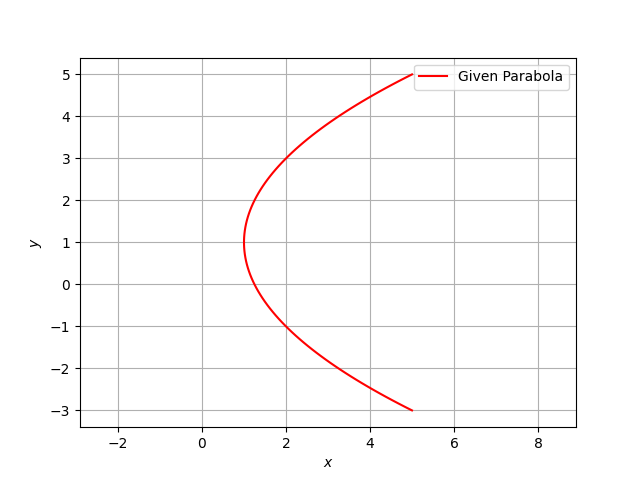
\includegraphics{figures/figure.png}}
    \caption{Plot of the locus}
\end{figure}
\end{document}
